% Caso 01 — Problema de Hill
\begin{frame}{Resultados — Caso 01: Problema de Hill}
    \textbf{Base del problema:} simplificación del problema restringido de 3 cuerpos; binaria + cuerpo ligero cercano al radio de Hill.
    \vspace{0.2cm}
    {\small
    \begin{itemize}
        \item Parámetros: $t_{short}=0.5$, $t_{long}=4.0$, $\Delta t=2\times10^{-4}$, integrador=\texttt{IAS15}.
        \item Masas originales (escenario base): $(1.3,\ 0.8,\ 1.3\times10^{-3})$.
        \item Posiciones iniciales $\mathbf{r}_0$ (UA): $(-0.09,0,0)$, $(0.11,0,0)$, $(0.52,0,0)$.
        \item Velocidades iniciales $\mathbf{v}_0$ (UA/año): $(0, 8.9411294392, 0)$, $(0,-10.9280470924,0)$, $(0,12.3223401880,0)$.
    \end{itemize}
    }
\end{frame}

\begin{frame}{Caso 01 — Masas optimizadas y comparativas}
    {\small
    \begin{itemize}
        \item Masas optimizadas: $(m_1, m_2, m_3) \approx (1.065762,\ 0.700000,\ 0.001200)$.
        \item Evolución de $\lambda$ (Lyapunov) y comparación de trayectorias.
    \end{itemize}}
    \vspace{0.2cm}
    \begin{columns}[T,totalwidth=\textwidth]
        \begin{column}{0.52\textwidth}
            \centering
            \adjustbox{max width=\linewidth, max height=0.7\textheight}{%
                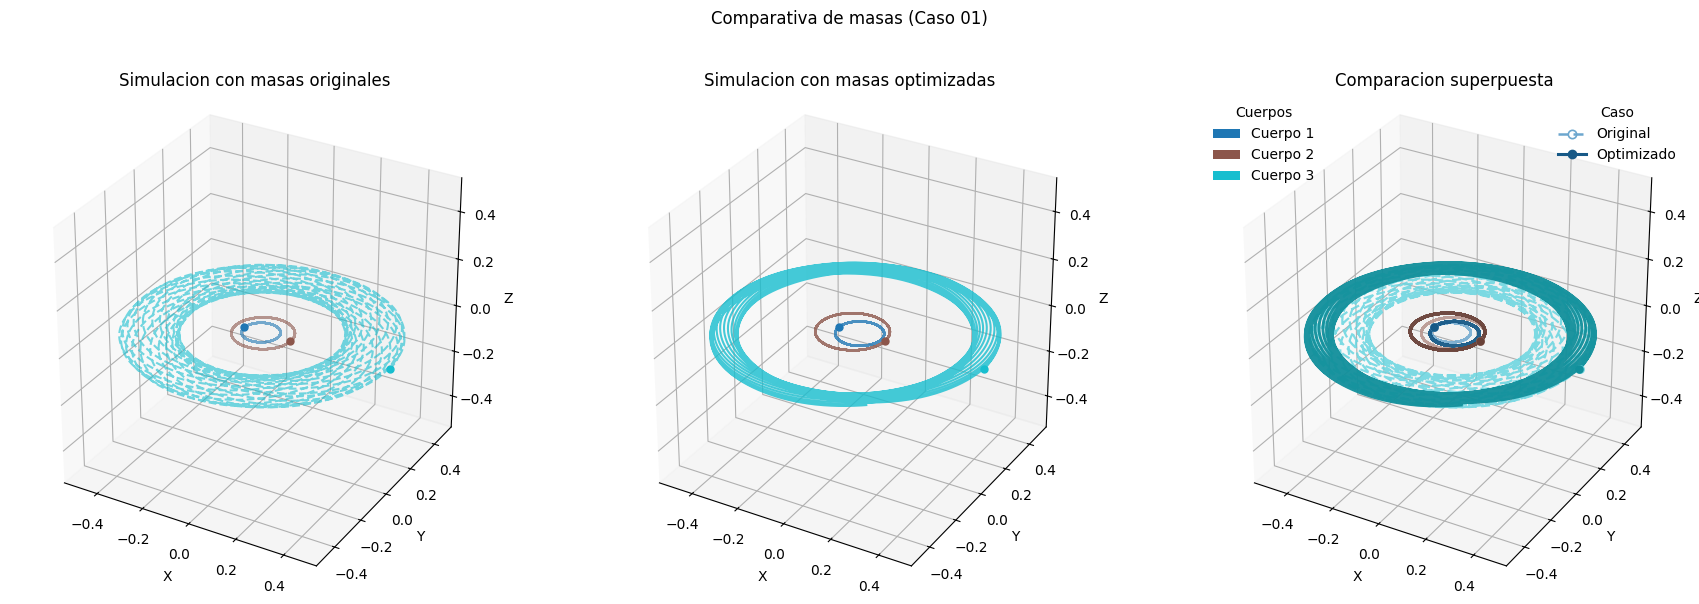
\includegraphics{img/resultados/caso01-comparativa_trayectoria.png}%
            }
            \\[-0.15cm]
            {\tiny Comparativa de trayectorias (original vs optimizada).}
        \end{column}
        \begin{column}{0.48\textwidth}
            \centering
            \adjustbox{max width=\linewidth, max height=0.7\textheight}{%
                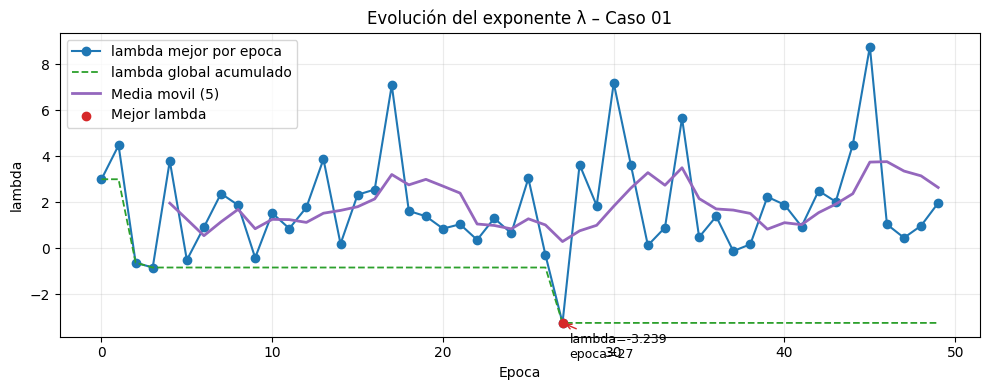
\includegraphics{img/resultados/caso01-evolucion_exponente.png}%
            }
            \\[-0.15cm]
            {\tiny Evolución del exponente de Lyapunov $\lambda$.}
        \end{column}
    \end{columns}
\end{frame}

